\section{Iterations}

The first two prototype ideas shown on figures \ref{fig:v1} and \ref{fig:v2} were made entirely with acrylic sheets cut with a laser-cutter. The figures show an exploded view of the design on left, and the physical version on the right. \\

The first prototype on figure \ref{fig:v1} was designed to accommodate eight banks of 4 x 1,5V AAA batteries. Compartments for each electronic component were made to place them on a flat surface, and reduce thickness. A box on the left of the journal was meant to hold LEDs. \\
This design had many flaws however -- the list below describes the various issues.

\begin{itemize} \itemsep0em
  \item It felt heavy, and the weight exceeded 500g.
  \item The sharp edges from the laser-cut acrylic were slightly uncomfortable.
  \item The sheets were glued together, and made it impossible to open in case of the need for maintenance.
  \item The glueing process is tedious, because of of the use of extra tools such as a clamp, and the hardening takes 24h.
  \item Compartments were engraved with the laser-cutter, which requires constant supervision of the cutting.
  \item Problems with displacement of compartments from the different acrylic sheets.
  \item No charging possibility.
  \item Wiring of components was difficult.
  \item The side piece made it difficult to open the journal.
\end{itemize}

A few positive characteristics were observed:
\begin{itemize} \itemsep0em
  \item Removal of protruding bolts.
  \item Reduced thickness by 15mm.
\end{itemize}

\clearpage

\begin{figure}[h]
\begin{minipage}[b]{7.5cm}
\centering
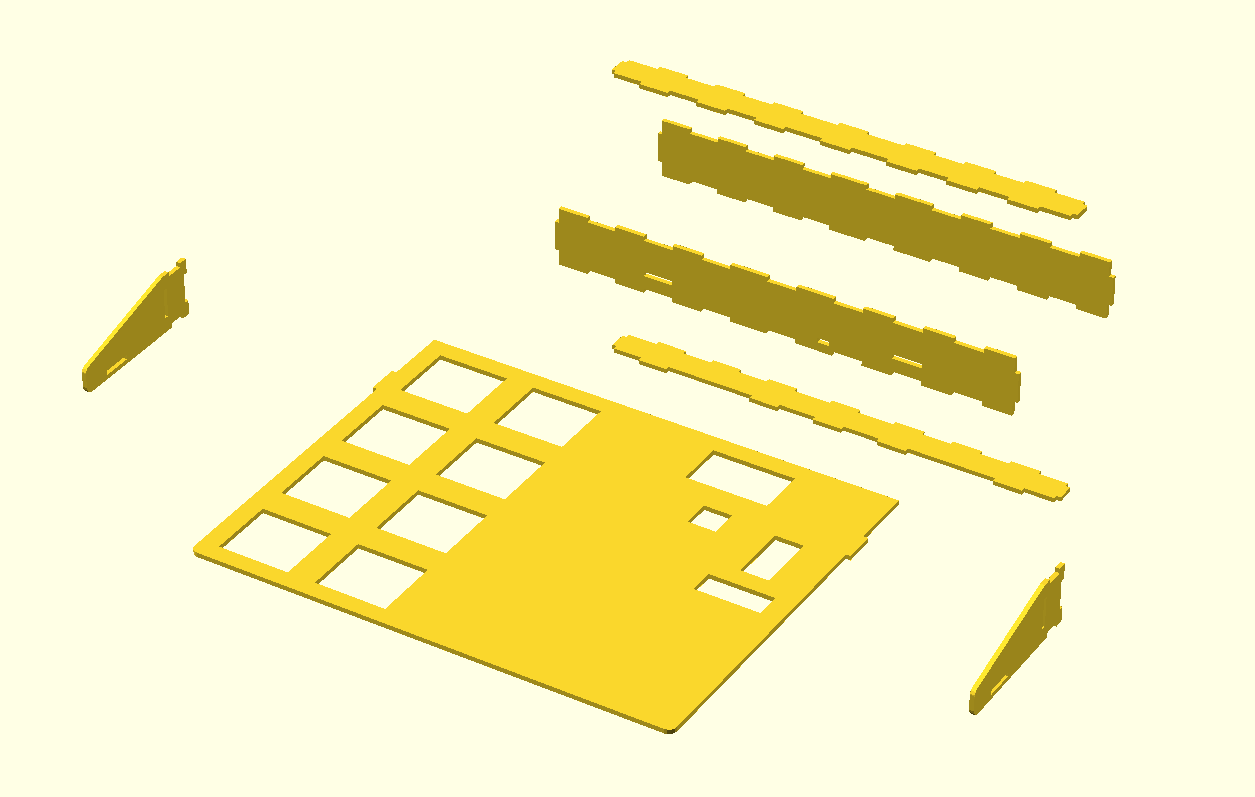
\includegraphics[scale=0.235]{figures/iterations/v1.png}
\end{minipage}
% \hspace{0.5cm}
\begin{minipage}[b]{7.5cm}
\centering
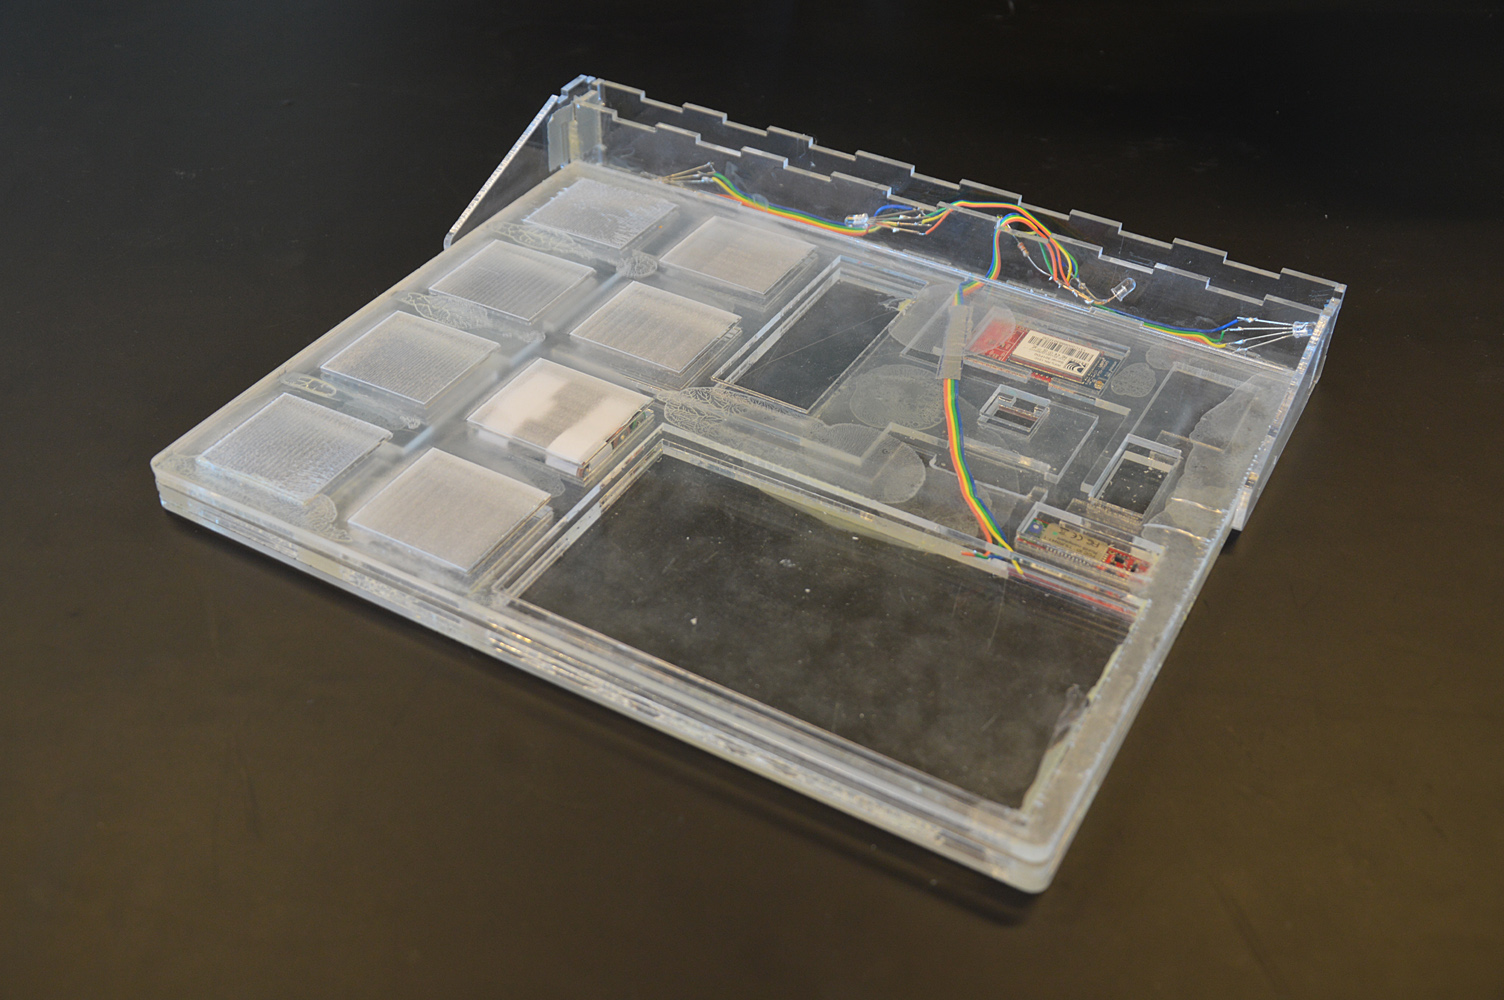
\includegraphics[scale=0.58]{figures/iterations/v1-photo.jpg}
\end{minipage}
\caption{\small {\it {The first prototype idea}}} \label{fig:v1}
\end{figure}

The second prototype took the previous downsides into consideration, and produced the device shown on figure \ref{fig:v2}. The downsides were assessed, and the electronics was then moved to a box at the bottom of the journal. 

\begin{figure}[h]
\begin{minipage}[b]{7.5cm}
\centering
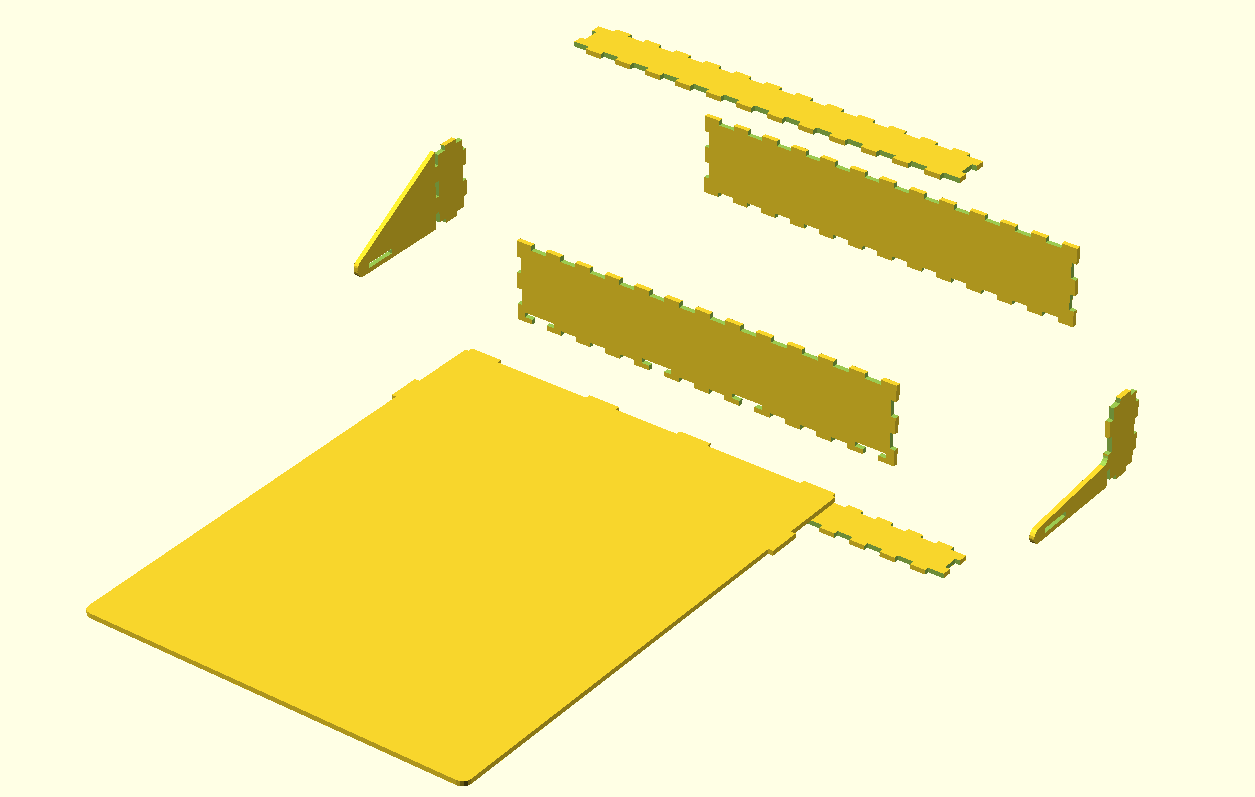
\includegraphics[scale=0.235]{figures/iterations/v3.png}
\end{minipage}
% \hspace{0.5cm}
\begin{minipage}[b]{7.5cm}
\centering
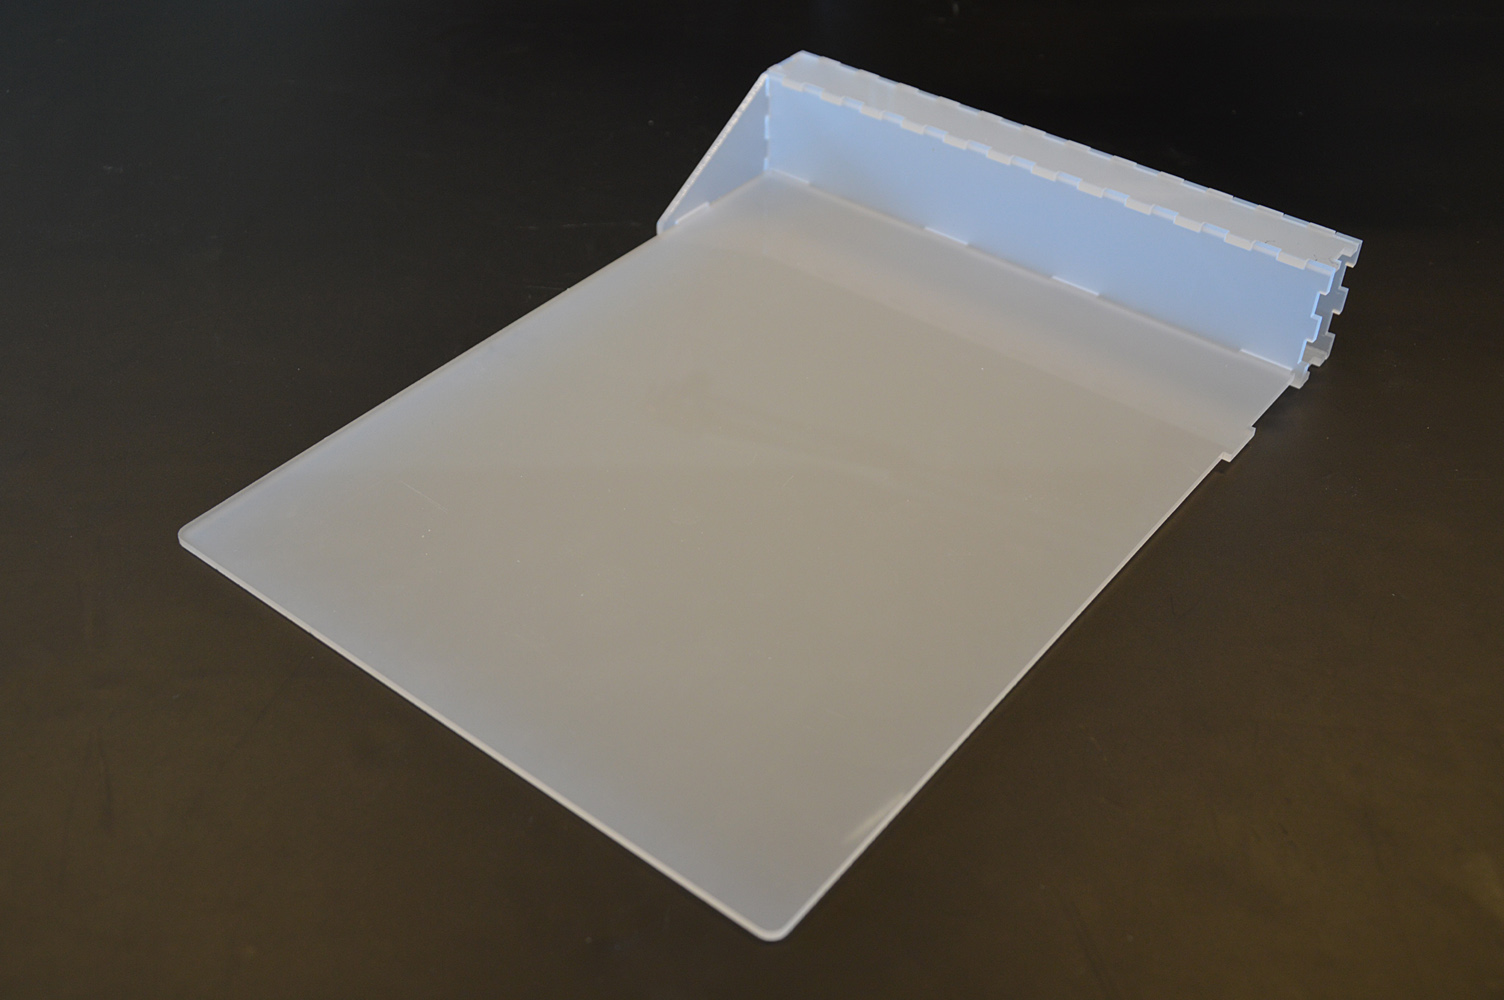
\includegraphics[scale=0.58]{figures/iterations/v3-photo.jpg}
\end{minipage}
\caption{\small {\it {The second prototype idea}}} \label{fig:v2}
\end{figure}


\begin{figure}[h]
\begin{minipage}[b]{7.5cm}
\centering
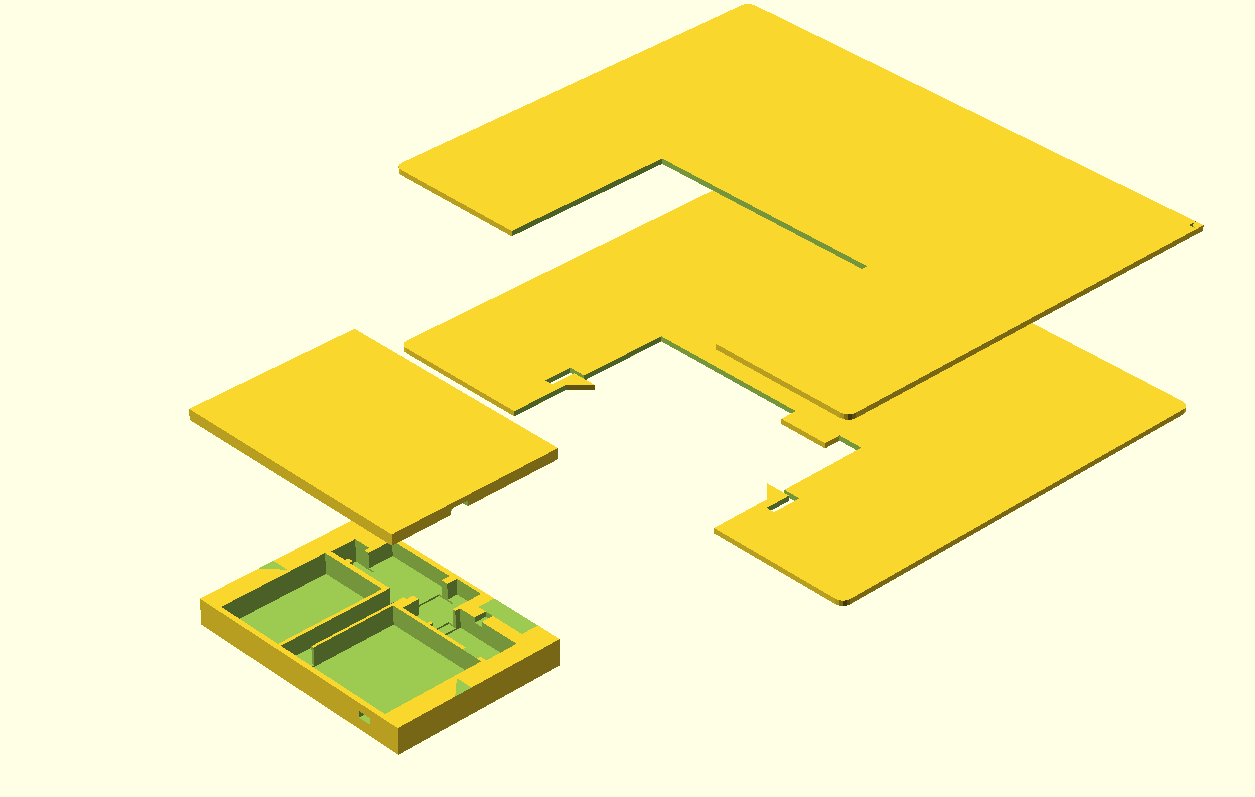
\includegraphics[scale=0.235]{figures/iterations/v4.png}
\end{minipage}
% \hspace{0.5cm}
\begin{minipage}[b]{7.5cm}
\centering
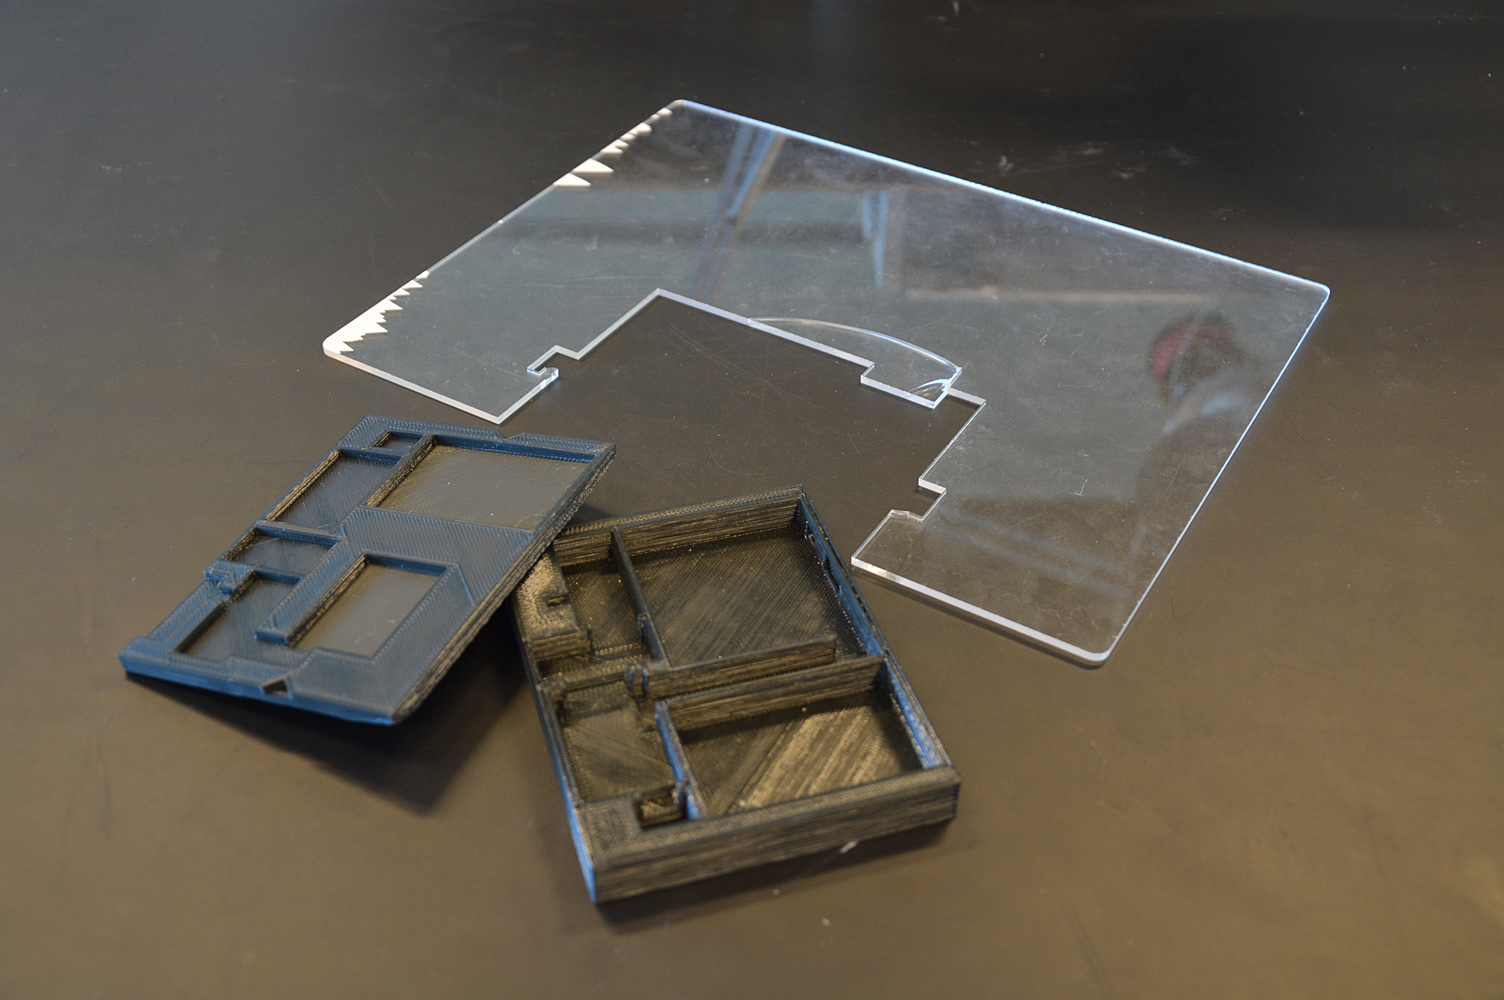
\includegraphics[scale=0.58]{figures/iterations/v4-photo.jpg}
\end{minipage}
\caption{\small {\it {The third prototype idea}}} \label{fig:v3}
\end{figure}


\begin{figure}[h]
\begin{minipage}[b]{7.5cm}
\centering
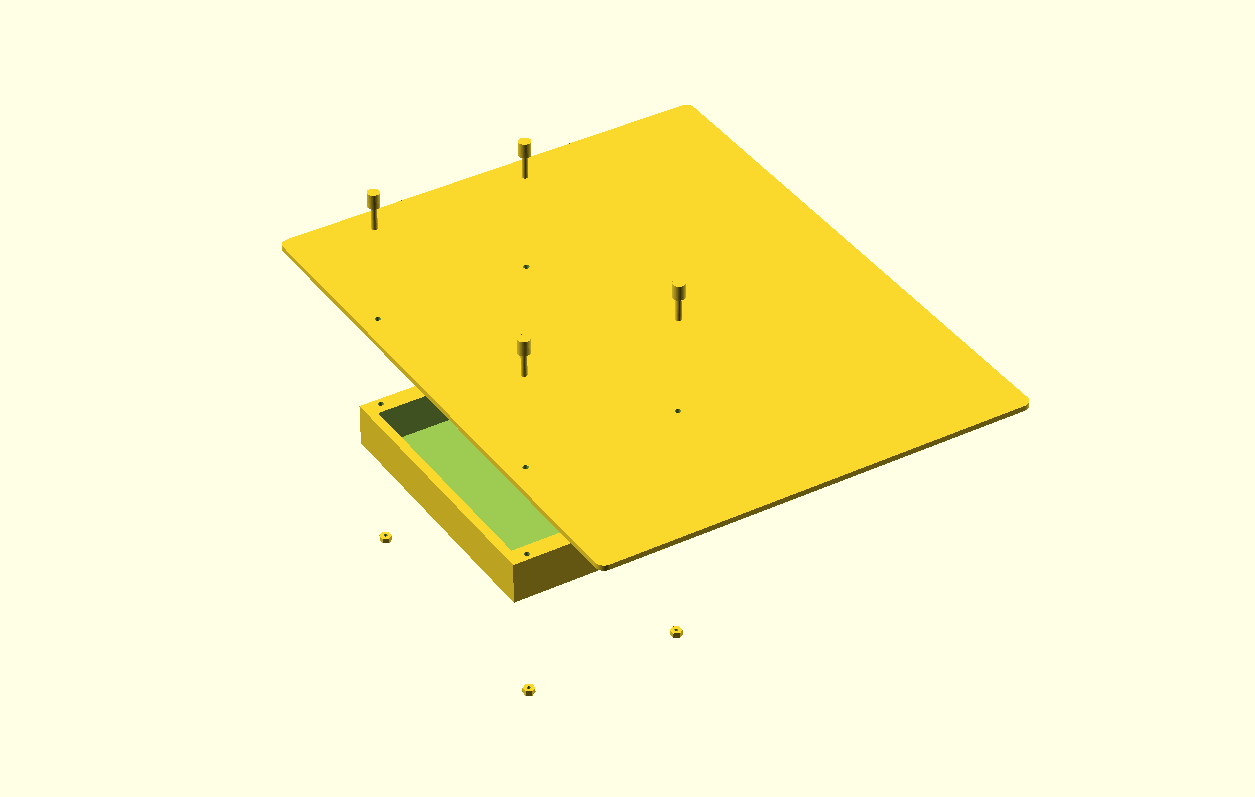
\includegraphics[scale=0.235]{figures/iterations/v5.png}
\end{minipage}
% \hspace{0.5cm}
\begin{minipage}[b]{7.5cm}
\centering
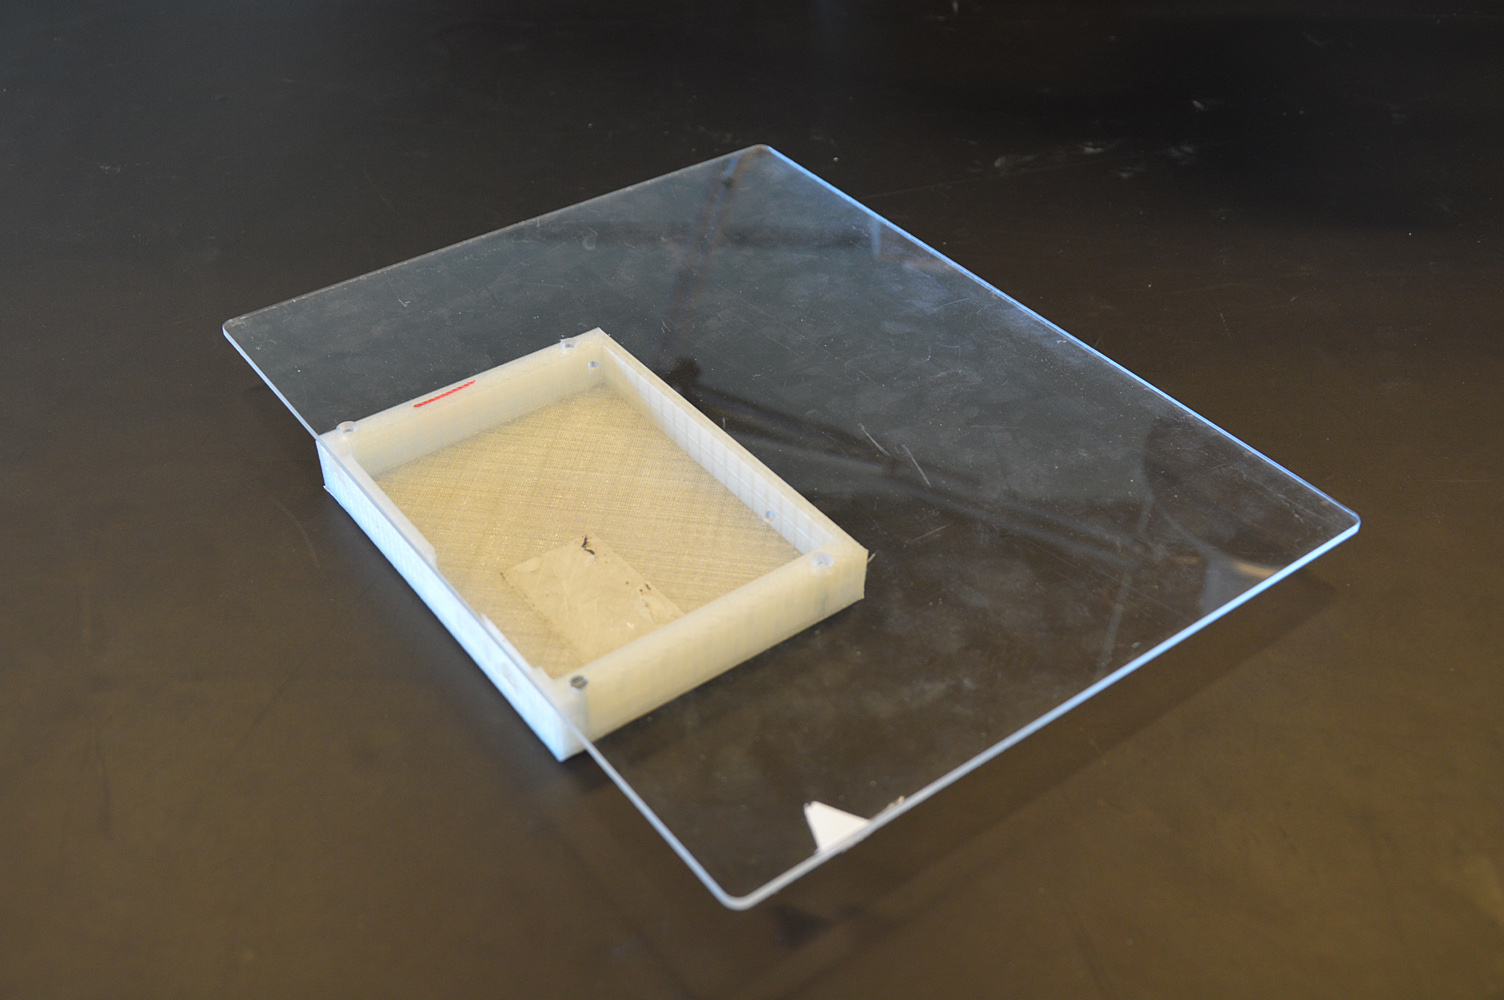
\includegraphics[scale=0.58]{figures/iterations/v5-photo.jpg}
\end{minipage}
\caption{\small {\it {The fourth prototype idea}}} \label{fig:v4}
\end{figure}


\begin{figure}[h]
\begin{minipage}[b]{7.5cm}
\centering
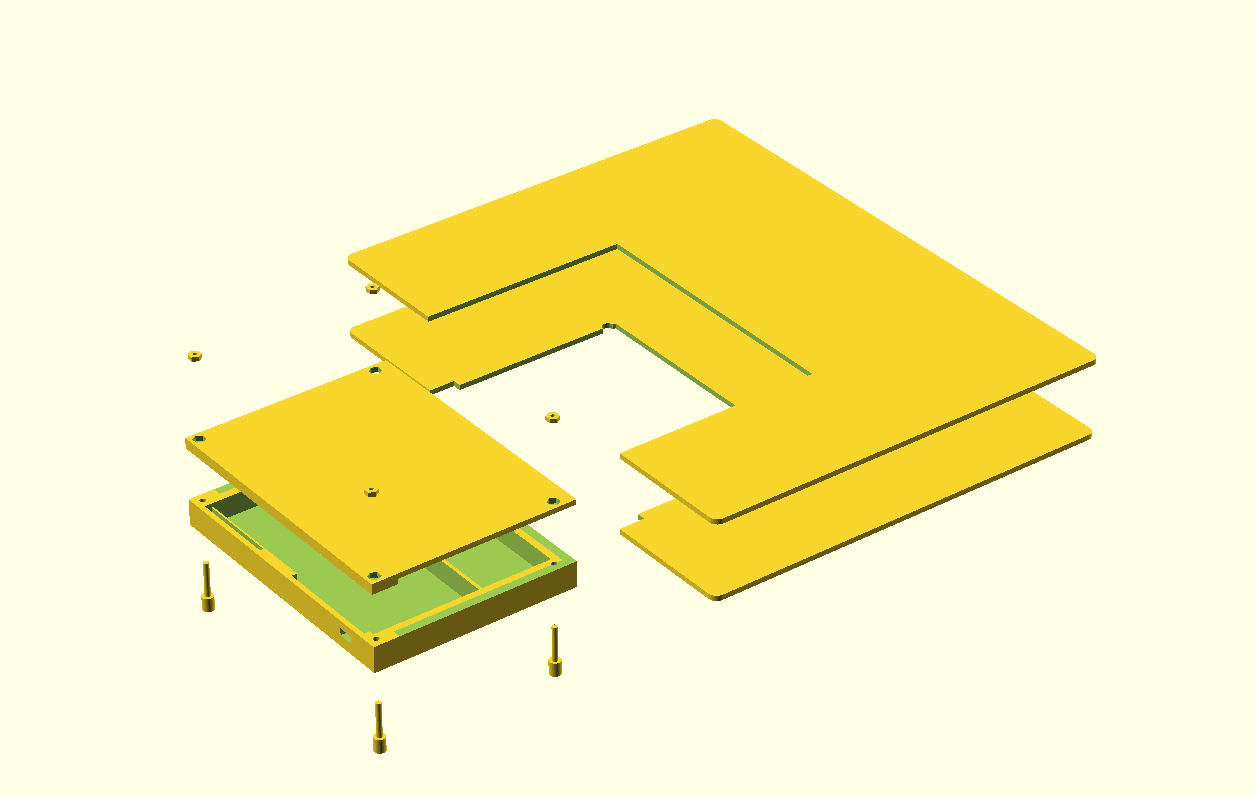
\includegraphics[scale=0.235]{figures/iterations/v6.png}
\end{minipage}
% \hspace{0.5cm}
\begin{minipage}[b]{7.5cm}
\centering
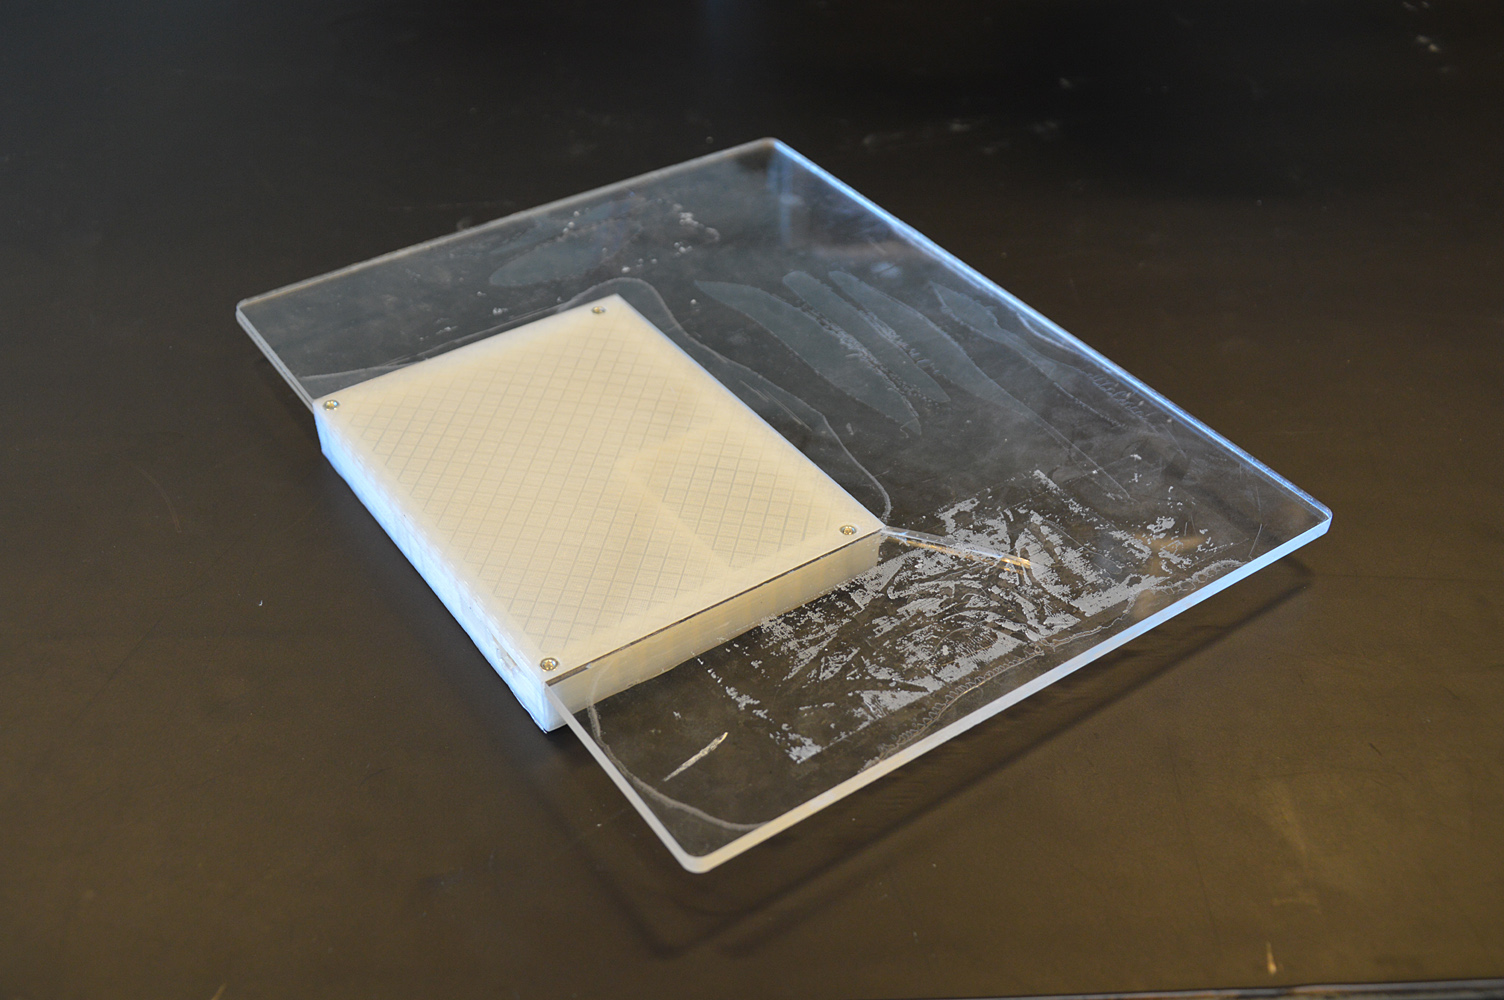
\includegraphics[scale=0.58]{figures/iterations/v6-photo.jpg}
\end{minipage}
\caption{\small {\it {The fifth prototype idea}}} \label{fig:v5}
\end{figure}



\clearpage